\documentclass[article]{IEEEtran}
\usepackage[a5paper, margin=10mm, onecolumn]{geometry}
%\usepackage{lmodern} % Ensure lmodern is loaded for pdflatex
\usepackage{tfrupee} % Include tfrupee package

\setlength{\headheight}{1cm} % Set the height of the header box
\setlength{\headsep}{0mm}     % Set the distance between the header box and the top of the text

\usepackage{gvv-book}
\usepackage{gvv}
\usepackage{cite}
\usepackage{amsmath,amssymb,amsfonts,amsthm}
\usepackage{algorithmic}
\usepackage{graphicx}
\usepackage{textcomp}
\usepackage{xcolor}
\usepackage{txfonts}
\usepackage{listings}
\usepackage{enumitem}
\usepackage{mathtools}
\usepackage{gensymb}
\usepackage{comment}
\usepackage[breaklinks=true]{hyperref}
\usepackage{tkz-euclide} 
\usepackage{listings}                                       
\def\inputGnumericTable{}                                 
\usepackage[latin1]{inputenc}                                
\usepackage{color}                                            
\usepackage{array}                                            
\usepackage{longtable}                                       
\usepackage{calc}                                             
\usepackage{multirow}                                         
\usepackage{hhline}                                           
\usepackage{ifthen}                                           
\usepackage{lscape}

\renewcommand{\thefigure}{\theenumi}
\renewcommand{\thetable}{\theenumi}
\setlength{\intextsep}{10pt} % Space between text and floats

\numberwithin{figure}{enumi}
\renewcommand{\thetable}{\theenumi}

% Marks the beginning of the document
\begin{document}
\bibliographystyle{IEEEtran}
\title{NCERT-9.6.11}
\author{EE24BTECH11035 - KOTHAPALLI AKHIL}
{\let\newpage\relax\maketitle}

\noindent\textbf{Question: }  
Solve the differential equation:  
\begin{align}
    y \, dx + (x - y^2) \, dy = 0.
\end{align}

\noindent\textbf{Solution:}  
Rewriting the equation:  
\begin{align}
    \frac{dy}{dx} = \frac{y^2 - x}{y}.
\end{align}
\begin{align}
    \frac{dy}{dx}+\frac{y}{x}=\frac{1}{x}.
\end{align}
Now, it is in the form of Bernoulli differential equation,\\
Integration factor(I.F) for above equation is
\begin{align}
  e^{\int \frac{1}{x} \, dx} = e^{\ln |x|}=|x|
\end{align}
Consider $x>0$, \\
solution of the equation is,
\begin{align}
    y(I.F)=\int{(I.F) \cdot \frac{1}{x} \, dx}
\end{align}
\begin{align}
    yx=\int{dx}
\end{align}
Now, on integrating we get,\\
\begin{align}
    yx=x+C
\end{align}
where C is constant of integration. Here we assume it as 0.\\
\vspace{0.5em}  

\noindent\textbf{Numerical Approach:}\\ 
I used a for loop for finding the $y$ values iteratively using the given formula. I initialized $x$ with a value and incremented it by $h$ in each iteration, where $h$ is the step size.  

\textbf{Using the Method of Finite Differences}\\ 
The Method of Finite Differences is a numerical technique used to approximate solutions to differential equations.  
We know that:  
\begin{align}
    \lim_{h \to 0} \frac{y(x+h) - y(x)}{h} = \frac{dy}{dx}.
\end{align}

For the given differential equation:  
\begin{align}
    \frac{dy}{dx} = \frac{y^2 - x}{y},
\end{align}

we approximate:  
\begin{align}
    \frac{y_{n+1} - y_n}{h} &\approx \frac{y_n^2 - x_n}{y_n}.
\end{align}

This implies:  
\begin{align}
    y_{n+1} &= y_n + h \cdot \frac{y_n^2 - x_n}{y_n}.
\end{align}

Here, $h$ is the step size, $y_n$ is the approximation of $y(x)$ at the $n$-th step, and $x_n$ is the corresponding $x$-value at the $n$-th step.  

\noindent The iterative formula for updating $y$-values is:  
\begin{align}
    y_n = y_{n-1} + h \cdot \frac{y_{n-1}^2 - x_{n-1}}{y_{n-1}},
\end{align}

The iterative formula for updating $x$-values is:  
\begin{align}
    x_n = x_{n-1} + h.
\end{align}

\noindent\textbf{Initial Conditions:}  
\begin{itemize}
    \item $x = 0.1$ (since \(x = 0\) leads to a division by zero)
    \item $y = 0$
    \item $h = 0.0002$
\end{itemize}

Using Matplotlib, I plotted the computed points and the graph of the exact solution to verify that they approximately match.  

\begin{figure}[h!]
\t\centering
\t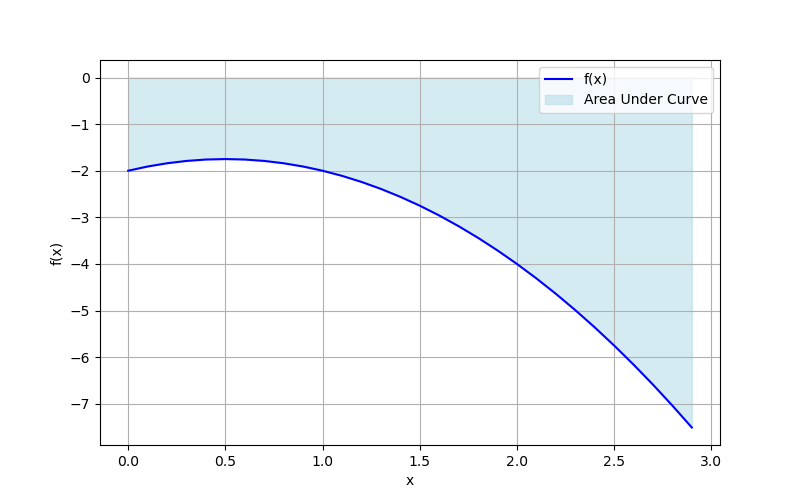
\includegraphics[width=\columnwidth]{figures/Figure_1.png}
\t\caption{verifying through graph of sim and theory values}
\t\label{stemplot}
\end{figure}

\end{document}

